\chapter{Using the ENRAM software}

Make sure you have your virtual machine running (as in Figure~\ref{fig:screenshot-19}). 

Start the File Manager by clicking on the desktop icon labeled `File Manager'. In the file manager window, double-click on the directory called `enram' to inspect its contents.

Start a terminal by double-clicking the desktop icon labeled `Terminal'. This should bring up a terminal program (Figure~\ref{fig:screenshot-24}).

Use the \texttt{cd} command to change directory into the `enram' directory.

\begin{figure}[ht]
  \centering
    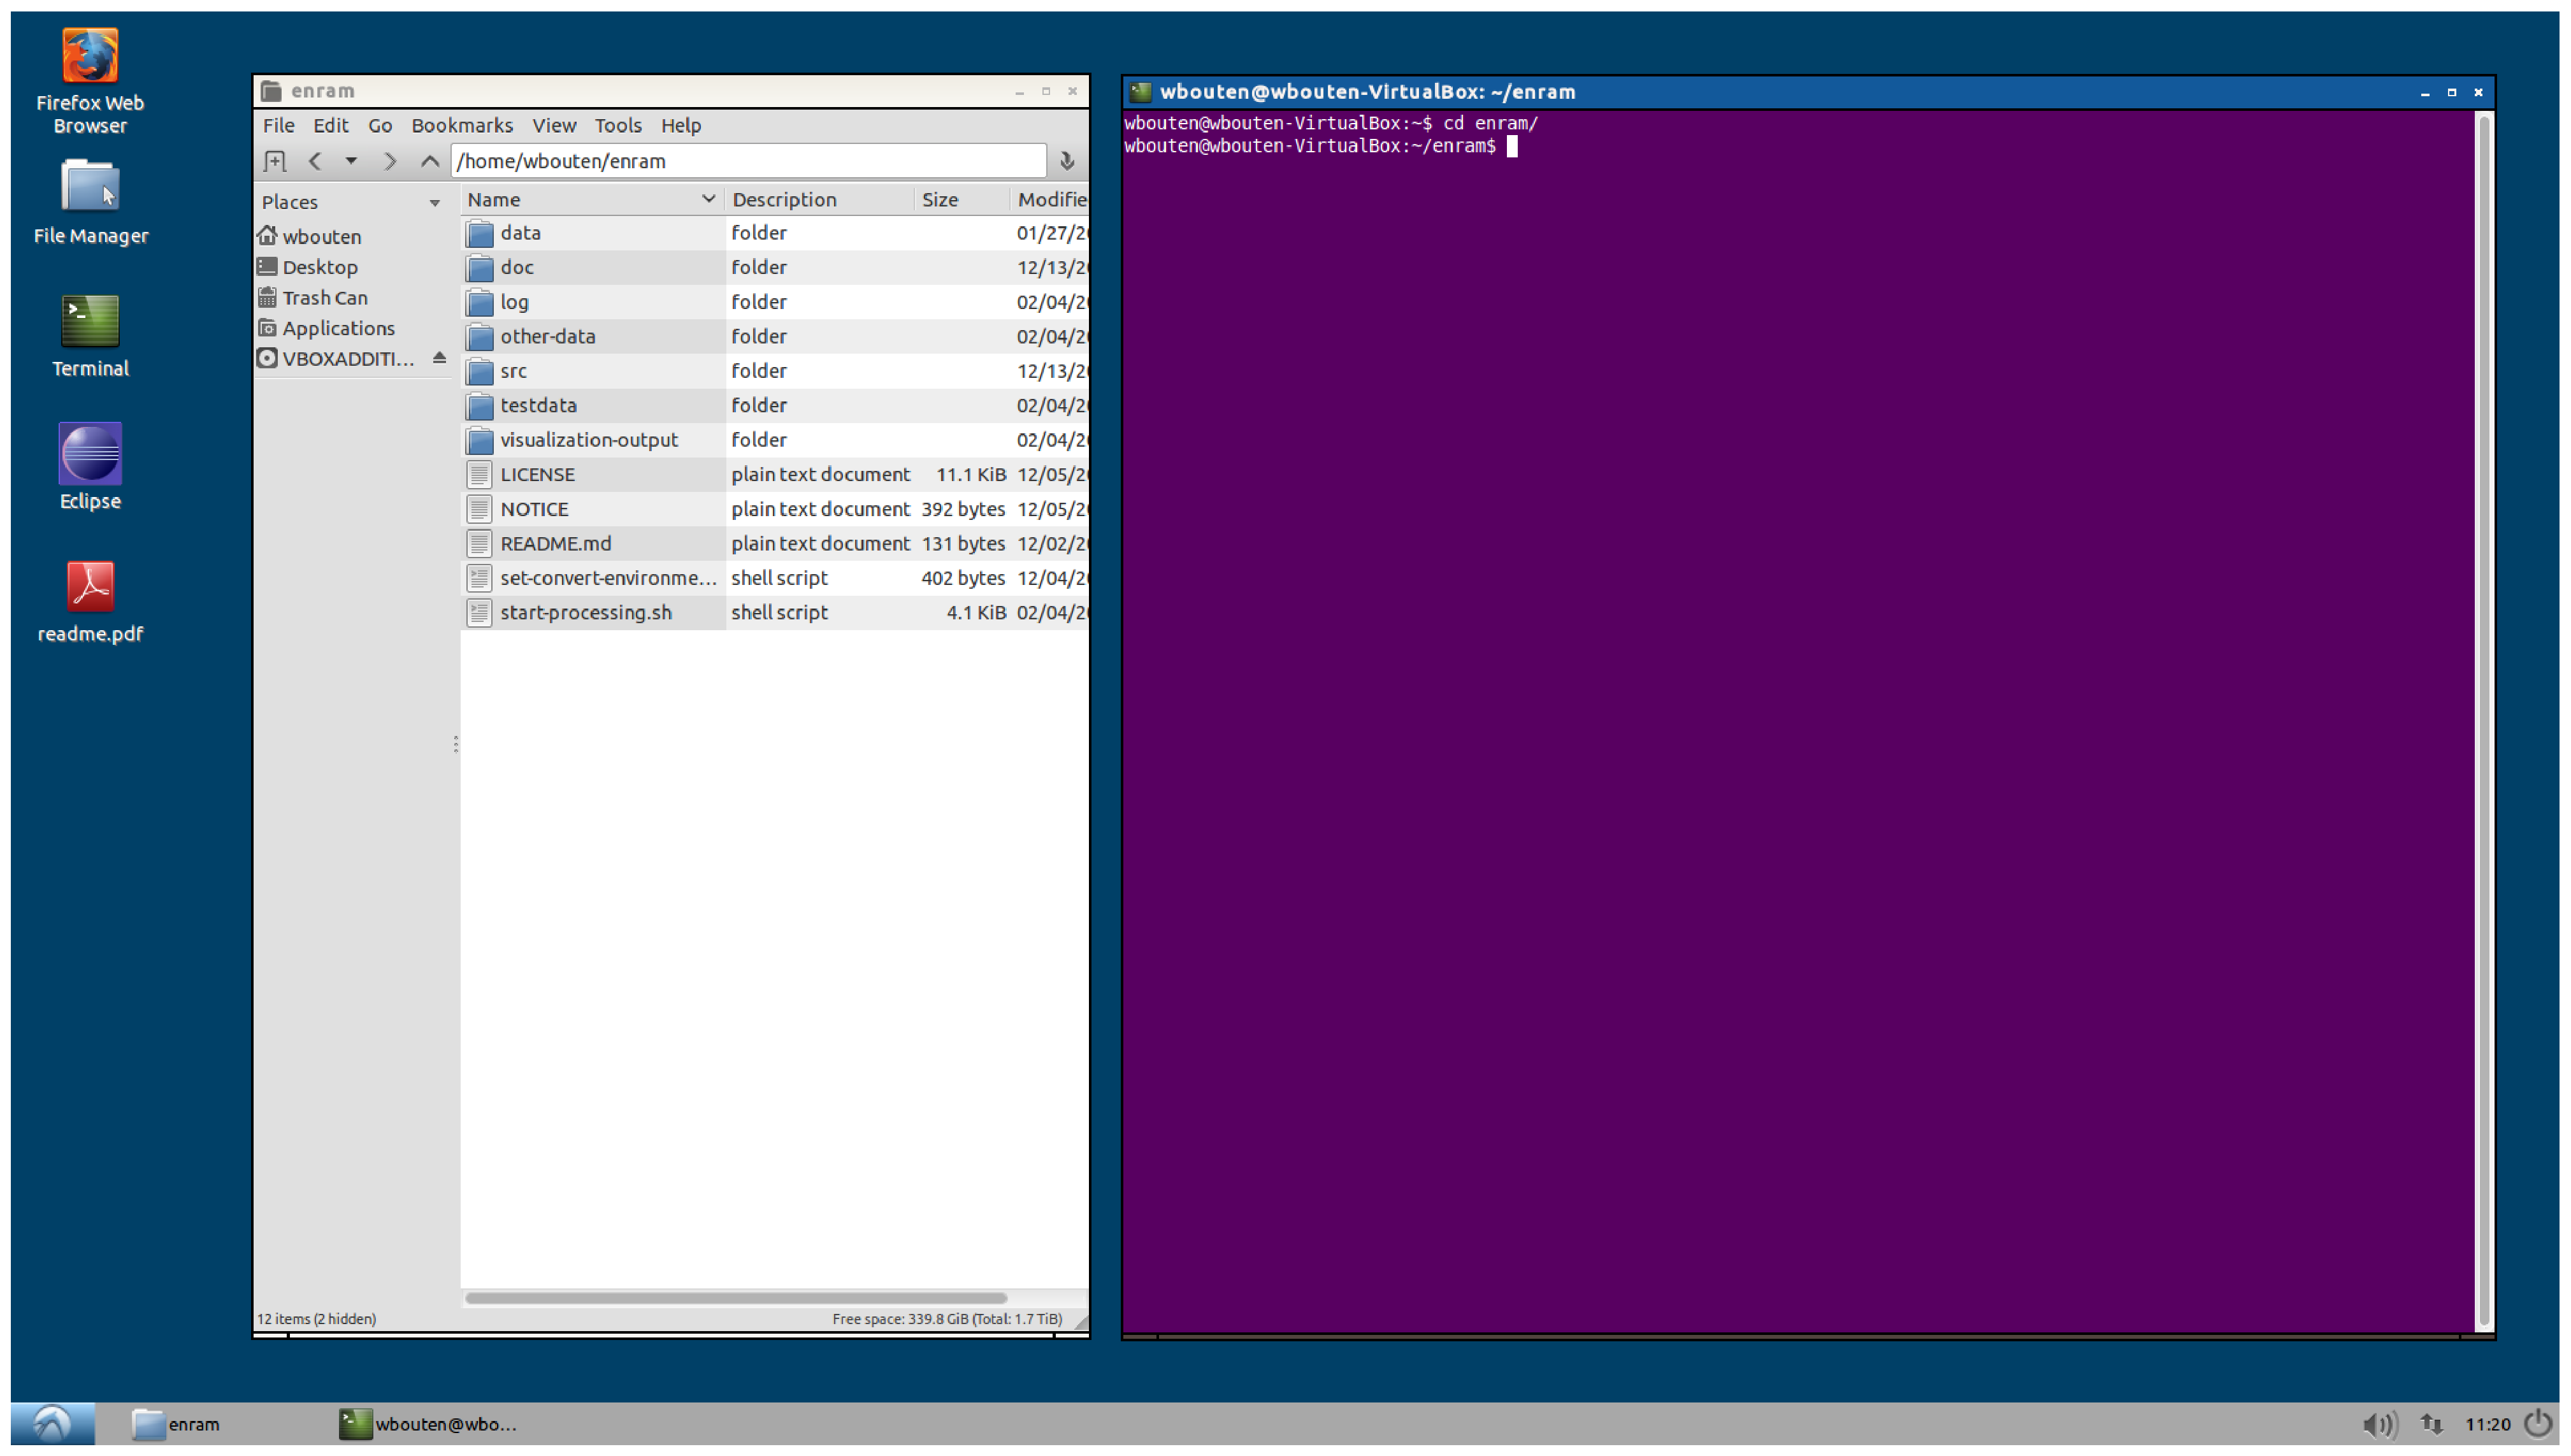
\includegraphics[width=0.85\linewidth , keepaspectratio]{./../eps/screenshot-24.eps}
  \caption{}
  \label{fig:screenshot-24}
\end{figure}
\clearpage

You can start the ENRAM workflow as follows. In the terminal window, type:\\
\texttt{. ./start-processing.sh}

(But make sure to type it exactly as it is displayed here, including the leading dot).

The terminal will then ask wether you want to run a test data set or the full data set (Figure~\ref{fig:screenshot-25}).

\begin{figure}[ht]
  \centering
    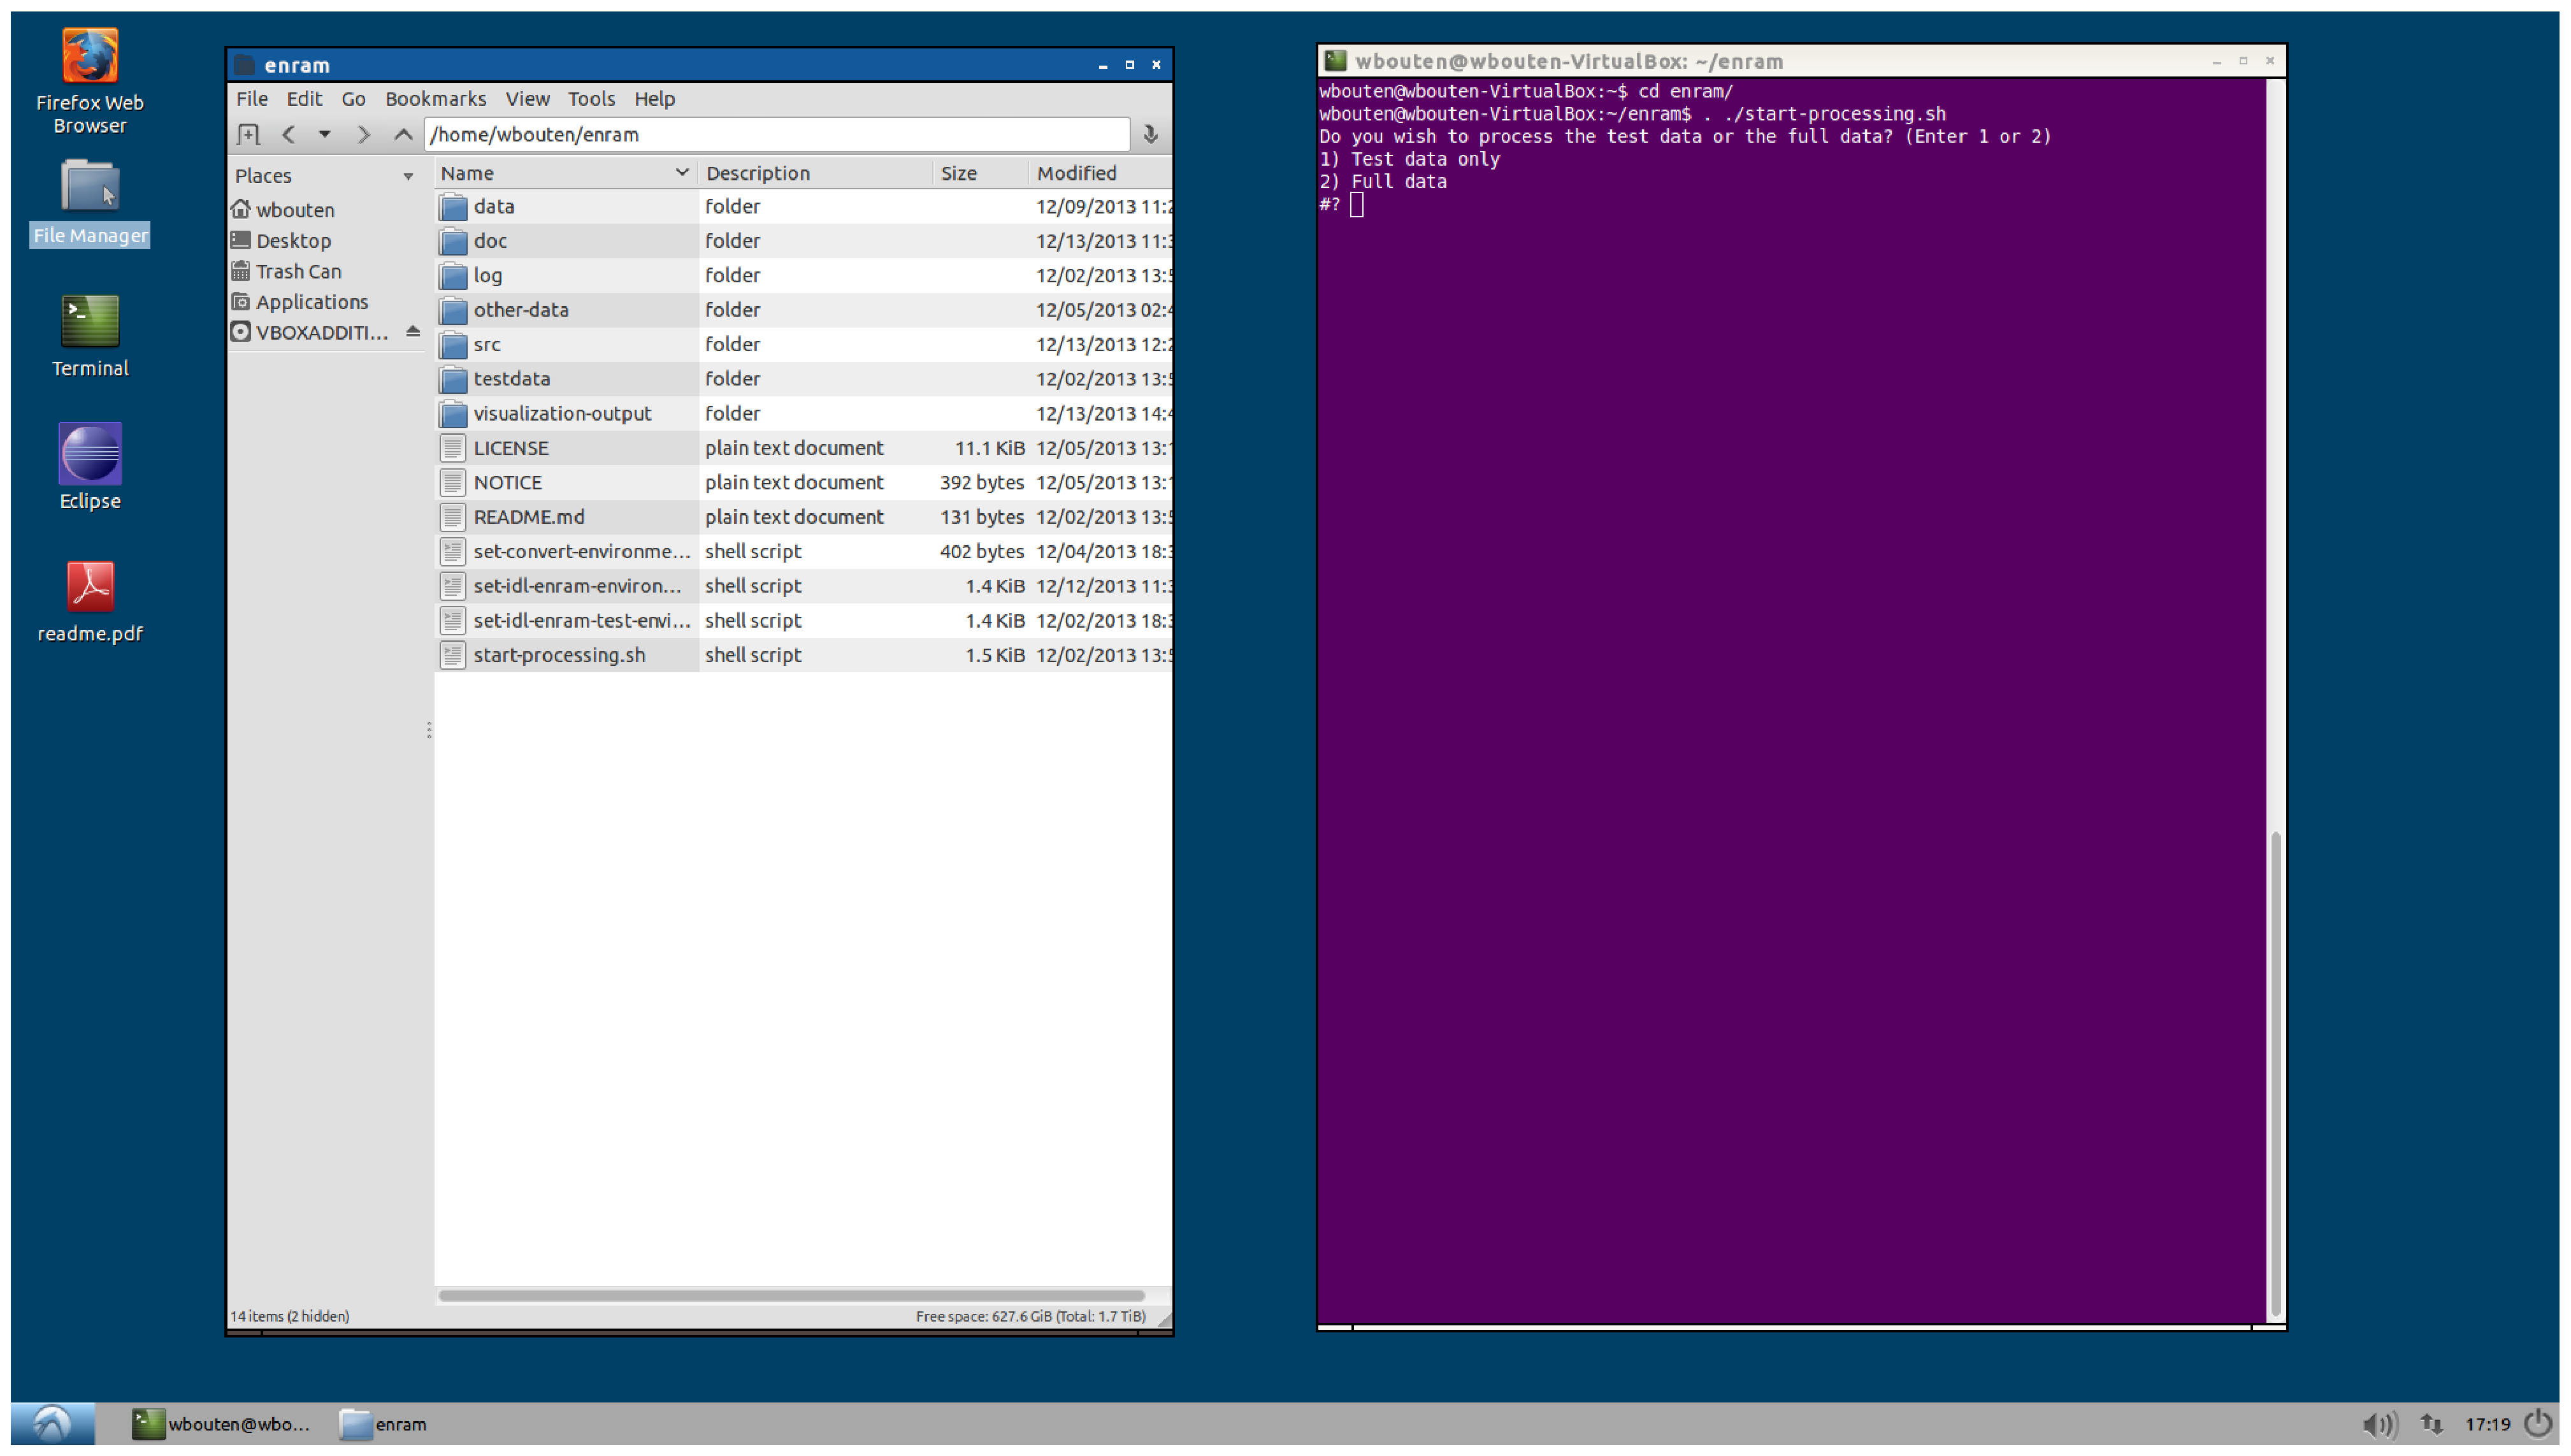
\includegraphics[width=0.85\linewidth , keepaspectratio]{./../eps/screenshot-25.eps}
  \caption{}
  \label{fig:screenshot-25}
\end{figure}

Answer `1' or `2' and press Enter. The terminal will now set up the right environment variables, and will subsequently start to run the ENRAM workflow. While the terminal program is running, you can use the browser to view the program's feedback (Figure~\ref{fig:screenshot-26}).


\begin{figure}[ht]
  \centering
    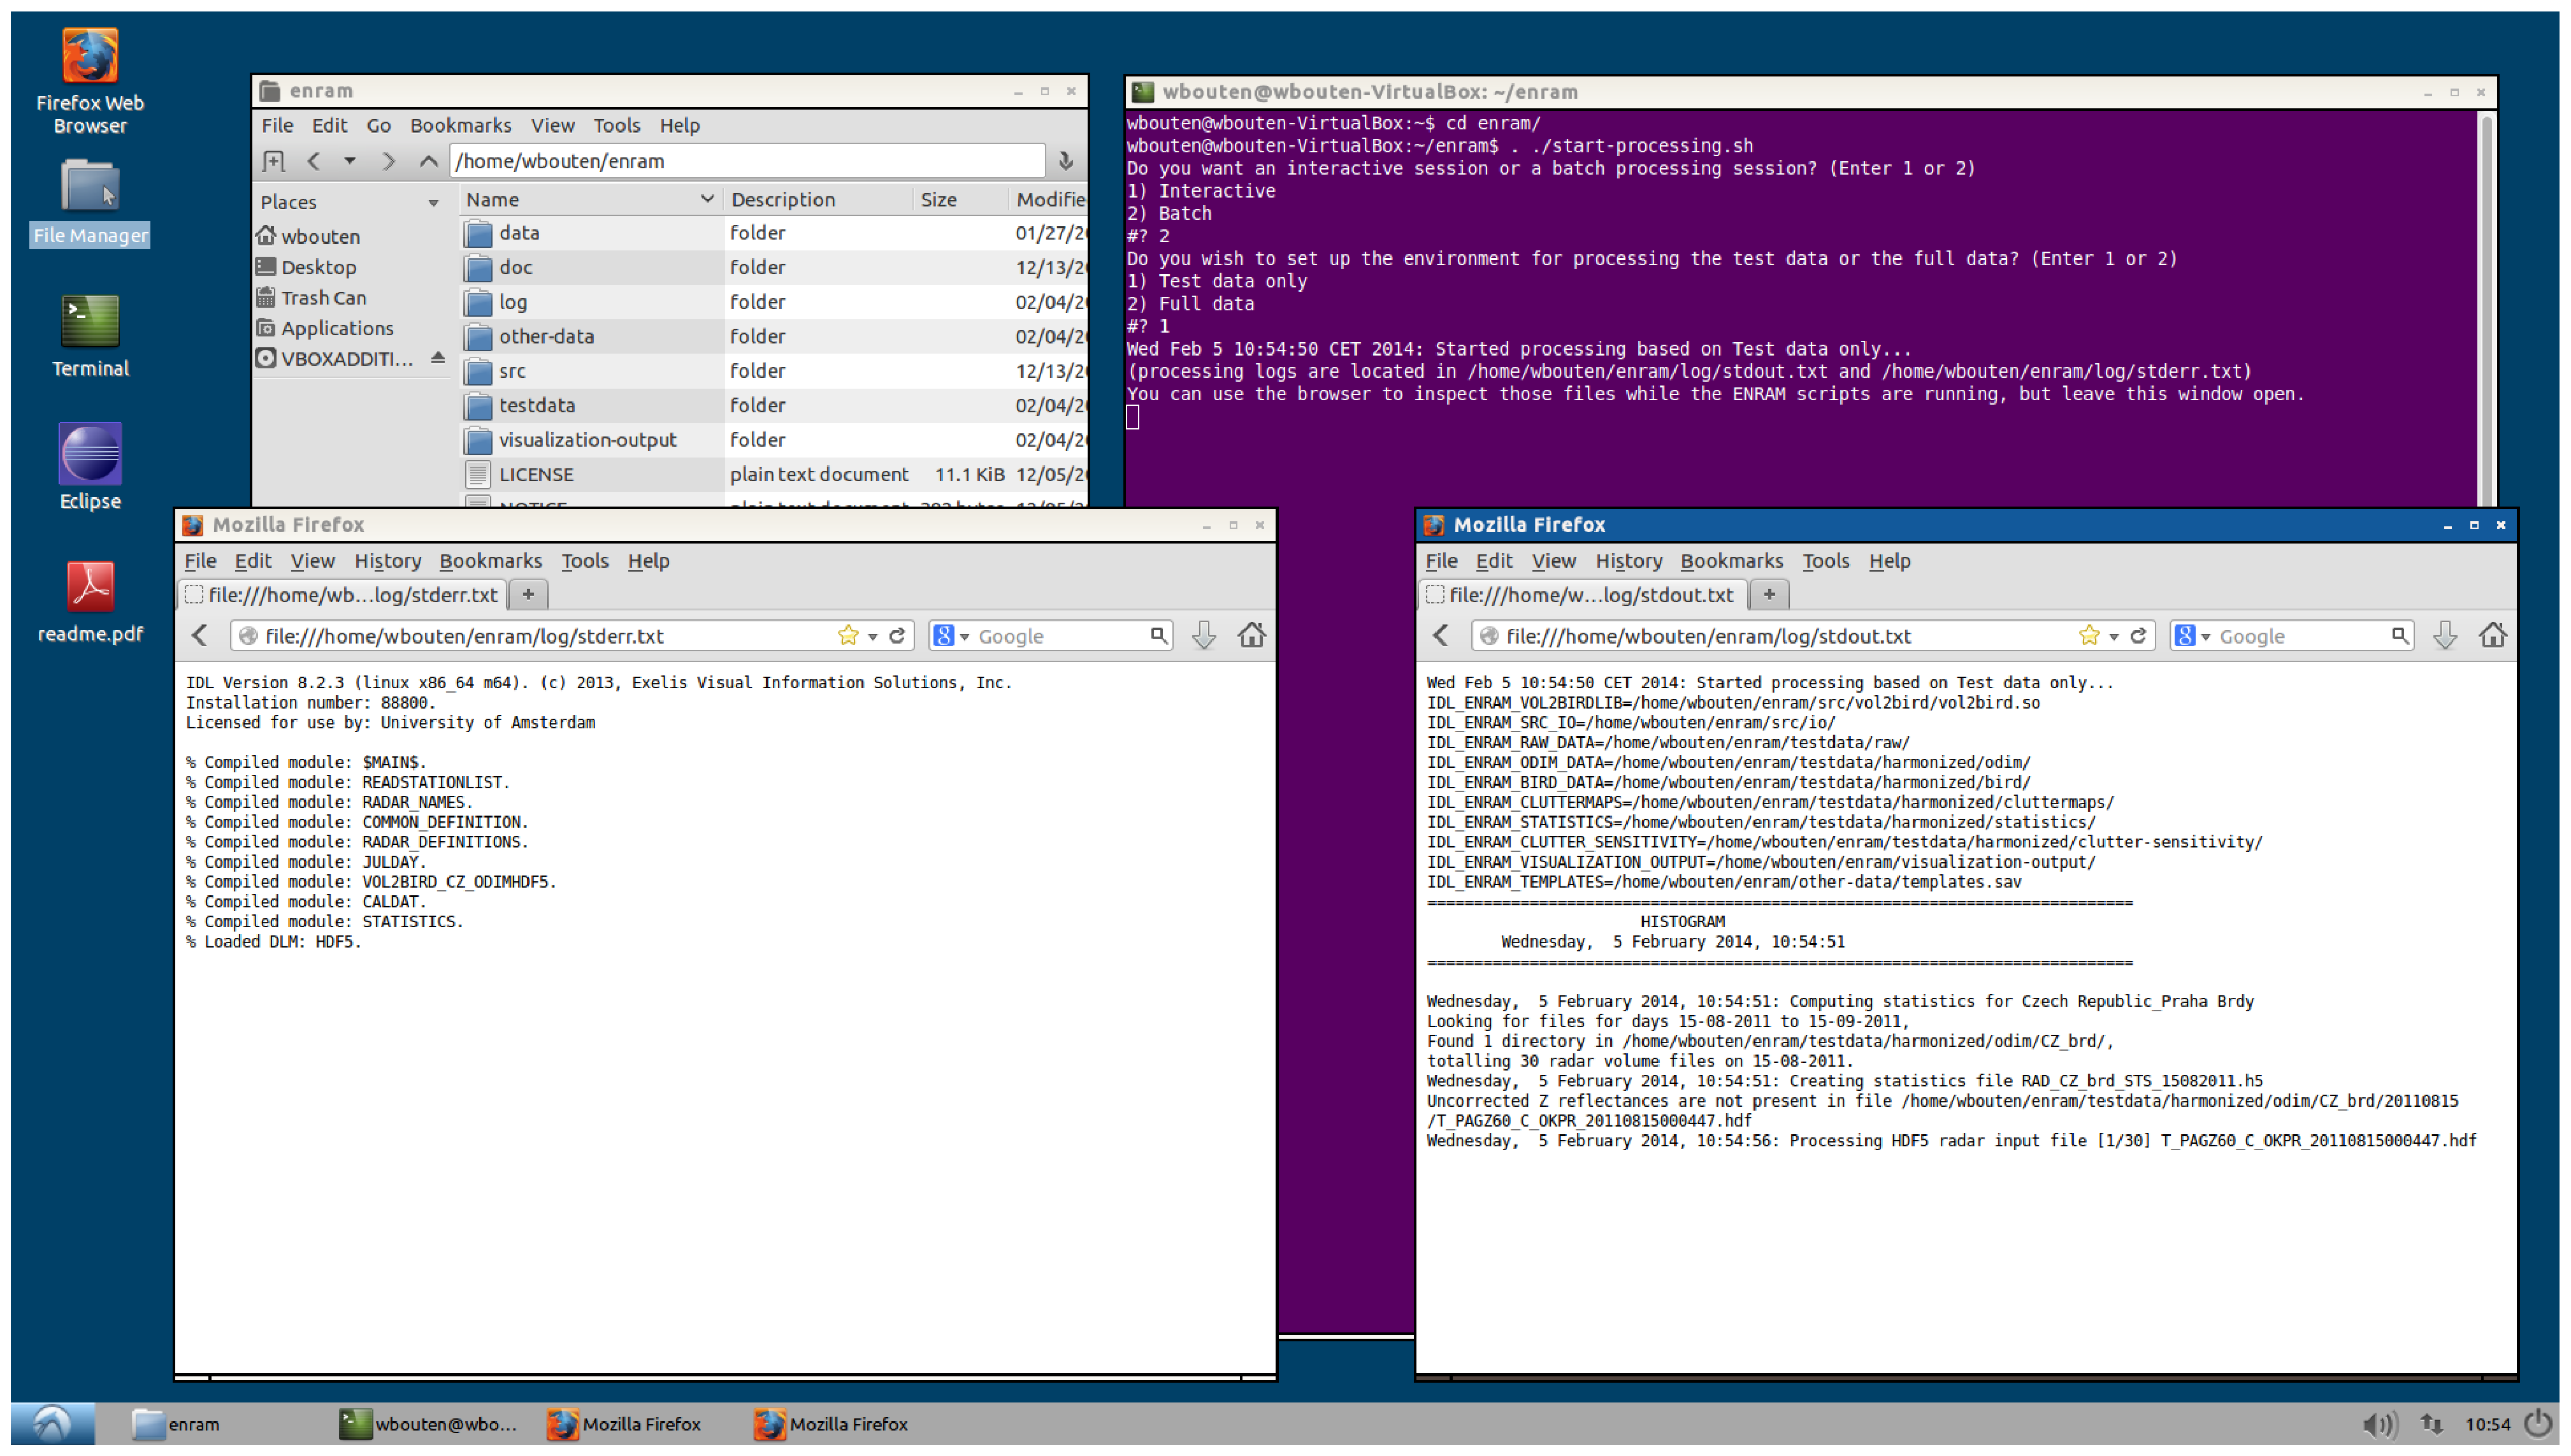
\includegraphics[width=0.85\linewidth , keepaspectratio]{./../eps/screenshot-26.eps}
  \caption{}
  \label{fig:screenshot-26}
\end{figure}
